% Aalto Master's Thesis template
% Compatible with: UTF-8, pdflatex, biblatex, biber
%
% Compile using the following commands:
% $ pdflatex thesis.tex
% $ biber thesis
% $ pdflatex thesis.tex
% $ pdflatex thesis.tex
% $ pdflatex thesis.tex
%

\documentclass[12pt,a4paper,oneside,pdftex]{report}

\usepackage[utf8]{inputenc}
\usepackage[T1]{fontenc}
\usepackage[finnish,swedish,english]{babel}
%\usepackage[english]{babel}


\usepackage{fancyvrb}%fancy verbatim
%\makeatletter
%\newcommand{\verbatimfont}[1]{\renewcommand{\verbatim@font}{\ttfamily\scriptsize#1}}
%\makeatother
% redefine \VerbatimInput
\RecustomVerbatimCommand{\VerbatimInput}{VerbatimInput}{fontsize=\scriptsize}

\usepackage{pmboxdraw}
\usepackage{newunicodechar}
\newunicodechar{└}{\textSFii}
\newunicodechar{├}{\textSFviii}
\newunicodechar{─}{\textSFx}


\usepackage{wrapfig} %for text wrap around figures
\usepackage{paracol}%2 columns

\usepackage[section]{placeins}

\usepackage{mathtools}
\usepackage{appendix}

\usepackage{fancyhdr}

\usepackage{mfirstuc}%title case

%\usepackage[final]{pdfpages}
\usepackage[export]{adjustbox} % loads also graphicx

%\newcommand{\pvec}[1]{\vec{#1}\mkern2mu\vphantom{#1}} %for primed vectors, see https://tex.stackexchange.com/a/120034
\newcommand{\pvec}[1]{\vec{#1}\,}

% Font selection
%\usepackage{palatino}
%\usepackage[sc]{mathpazo}
\usepackage{kpfonts}
%\usepackage{tgpagella}
%\usepackage{garamond}
%\usepackage{lmodern}

% Verbatim provides a standard teletype environment that renderes
% the text exactly as written in the tex file. Useful for code
% snippets (although you can also use the listings package to get
% automatic code formatting).
\usepackage{verbatim}
\usepackage{enumitem} % for nolistsep in enumeration
\usepackage{multicol} % for using multiple columns in listings

\usepackage{listings}
\usepackage{inc/listingset}


\renewcommand{\labelitemii}{$\circ$}

\lstset{ 
    columns=[l]fullflexible,
    keepspaces=true,
    basicstyle=\ttfamily\small,
    %numbers=left,
    tabsize=2,
    captionpos=b,
    escapeinside={[*}{*]},
}
\newcommand{\tool}[1]{#1}%{\texttt{#1}}

\newcommand*{\fx}{\ensuremath{\mathbf{x}}}%x}}}
\newcommand*{\fv}{\ensuremath{\mathbf{v}}} %v}}}

\newcommand{\porthos}[1][]{%\texttt{%
Porthos\ifthenelse%
{\equal{#1}{}}%if
{}%then
{\ifthenelse{\equal{#1}{1}}%else-if
{\,v1}%then
{%else
\ifthenelse{\equal{#1}{2}}%else-if
{C}%then
{#1}%else
}}}%}
\newcommand{\oldporthos}{\porthos[1]}
\newcommand{\rf}{\ensuremath{\,\mathtt{rf}\,}}
\newcommand{\fr}{\ensuremath{\,\mathtt{fr}\,}}
\newcommand{\po}{\ensuremath{\,\mathtt{po}\,}}
\newcommand{\co}{\ensuremath{\,\mathtt{co}\,}}
\newcommand{\com}{\ensuremath{\,\mathtt{po}\,}}
\newcommand{\sr}{\ensuremath{\,\mathtt{sr}\,}}
\newcommand{\cat}{CAT}
\newcommand{\relation}[1]{\ensuremath{\overset{\mathtt{#1}}{\rightarrow}}}
\newcommand{\rel}[1]{\texttt{#1}}
\newcommand{\mathr}[1]{\ensuremath{\mathtt{#1}}}
\newcommand{\invrel}[1]{\ensuremath{\mathr{#1}\!\!\mathbin{\char`\^}\!\!\text{-1}}} %inversion or a relation in math mode: r^-1
\newcommand{\relminus}{\!\smallsetminus\!}

\makeatletter
\newcommand*{\defeq}{\mathrel{\rlap{%
                     \raisebox{0.3ex}{$\m@th\cdot$}}%
                     \raisebox{-0.3ex}{$\m@th\cdot$}}%
                     =}
\makeatother


\newcommand{\ytree}{\ensuremath{\text{Y-tree}}}
\newcommand{\wmodel}{\ensuremath{\text{W-model}}}%\mathtt{W\text{-}model}}}
\newcommand{\zformula}{\ensuremath{\text{Z-formula}}}
\newcommand{\xgraph}[1][]{\ensuremath{\text{X-graph}
\ifthenelse%
{\equal{#1}{}}%if
{}%then
{_{\text{\tiny{#1}}}}%else
}}
\newcommand{\xgraphU}[1][]{\ensuremath{\text{X-graph}%\mathtt{X\text{-}graph%unrolled x-graph
\ifthenelse%
{\equal{#1}{}}%if
{}%then
{_{\text{\tiny{#1}}}^{\text{\tiny{U}}}}%else
}}

\sloppy %forbid page overfull with texttt words

\usepackage{outlines} %for nested itemize lists

% Longtable provides a tabular environment that can span multiple
% pages. This is used in the example abbreviations file.
\usepackage{longtable}

% The titlesec package can be used to alter the look of the titles
% of sections, chapters, and so on. This example uses the ``medium''
% package option which sets the titles to a medium size, making them
% a bit smaller than what is the default. You can fine-tune the
% title fonts and sizes by using the package options. See the package
% documentation.
%\usepackage[medium]{titlesec}
\usepackage[medium,raggedright]{titlesec}
%\usepackage{pxfonts} %for listings

\usepackage[position=b]{subcaption}
\captionsetup[subfigure]{font=scriptsize,justification=centering}
\usepackage{graphicx}

\usepackage{tikz}
\usetikzlibrary{positioning}
\usetikzlibrary{calc}
\usetikzlibrary{arrows}
\usetikzlibrary{decorations.pathmorphing,decorations.markings}
\usetikzlibrary{shapes}
\usetikzlibrary{patterns}
\usetikzlibrary{automata}

\tikzset{initial text={}}
%\tikzset{%
%  zeroarrow/.style = {-stealth,dashed},
%  onearrow/.style = {-stealth,solid},
%  c/.style = {circle,draw,solid,
%    minimum width=3cm,
%    minimum height=3cm,
%    },
%  r/.style = {rectangle,draw,solid,minimum width=2em,
%    minimum height=2em}
%}
\tikzset{
c/.style={
  circle,solid,
  inner sep=0pt,
  %text width=1mm,
  minimum width=7mm,
  align=center,
  draw=black,
  fill=white
  }
}

\usepackage{amsthm}
\theoremstyle{definition}
\newtheorem{definition}{Definition}[section]

\usepackage{algorithm}
\usepackage[noend]{algpseudocode}
\renewcommand{\algorithmicrequire}[1]{\textbf{Input:} {#1}\\}
\renewcommand{\algorithmicensure}[1]{\textbf{Output:} {#1}}
\renewcommand{\algorithmicforall}{\textbf{for each}}
\newcommand{\Break}{\State\algorithmicbreak}

% Microtype for better typography
\usepackage[stretch=30,protrusion=true,final,expansion,tracking=true,kerning,spacing]{microtype}

% SI units. See table in 2lorem.tex for example
\usepackage{siunitx}
\sisetup{
    alsoload=binary
}

% Publication quality tables. See table in 2lorem.tex for example
\usepackage{booktabs}
% Use biber instead of bibtex as it supports UTF-8 among other things
\usepackage[backend=biber,
%maxnames=5,
%style=numeric-verb,
style=alphabetic,%-verb,%style=alphabetic
minalphanames=3,
maxalphanames=3,
maxbibnames=5, minbibnames=5, %for 'et al'
%sortcites=true,
%sorting=none
%see options: http://texdoc.net/texmf-dist/doc/latex/biblatex/biblatex.pdf
%sorting=anyvt,%Sort by alphabetic label, name, year, volume, title,
sorting=anyvt,%Sort by alphabetic label, name, year, title,
%sorting=ydnt,%Sort by year (descending), name, title 
%sorting=ynt, %Sort by year, name, title. 
%sorting=nyt, %Sort by name, year, title. %see https://tex.stackexchange.com/a/51439
]{biblatex}
% A catch-all filter for all items which are not assigned to a dedicated sub-bibliography:
%\defbibfilter{other}{
%  not type=article
%  and
%  not type=book
%  and
%  not type=collection
%}
%make the plus sign in bibliography references as superscript:
\renewcommand*{\labelalphaothers}{\textsuperscript{+}}


% Separate multiple citations with space instead of comma
% E.g. "[1] [2] [3]" instead of "[1], [2], [3]"
%\renewcommand\multicitedelim{\space}
%separate them by semicolon
%\renewcommand*{\multicitedelim}{\setunit{; }}


% Nicer looking caption for figures, tables, etc.
\usepackage[labelfont={bf},textfont={it},justification={raggedright},singlelinecheck={false}]{caption}

% Multiple figures inside one figure. See figure in 1lipsum.tex for example
%\usepackage{subfig}

% Inconsolata monospace font for verbatim environment
\usepackage{inconsolata}

% For rotating figures
\usepackage{rotating}

\usepackage{hyphenat} % for using \nohyphens

% Prevent orphan and widow rows
\widowpenalty=10000
\clubpenalty=10000

% Bibliography
\addbibresource{bib/ms-thesis.bib}

\usepackage[doublenumbering,twosupervisors]{lib/aalto-thesis}


% Hyperref
% ------------------------------------------------------------------
% Hyperref creates links from URLs, for references, and creates a
% TOC in the PDF file.
% This package must be the last one you include, because it has
% compatibility issues with many other packages and it fixes
% those issues when it is loaded.
\RequirePackage[pdftex]{hyperref}
% Setup hyperref so that links are clickable but do not look
% different
\hypersetup{colorlinks=false,raiselinks=false,breaklinks=true}
\hypersetup{pdfborder={0 0 0}}
\hypersetup{bookmarksnumbered=true}
% The following line suggests the PDF reader that it should show the
% first level of bookmarks opened in the hierarchical bookmark view.
\hypersetup{bookmarksopen=true,bookmarksopenlevel=1}
% Hyperref can also set up the PDF metadata fields. These are
% set a bit later on, after the thesis setup.

\newcommand{\TITLE}{\nohyphens{Automated Analysis of Weak Memory Models}}
%\newcommand{\FTITLE}{?}
%\newcommand{\FSUBTITLE}{}
%\newcommand{\FDATE}{?.?.2018} % TODO
\newcommand{\SUBTITLE}{}
\newcommand{\DATE}{18.6.2018}

% Supervisors and instructors
% ------------------------------------------------------------------
% If you have two supervisors, write both names here, separate them with a
% double-backslash (see below for an example)
% Also remember to add the package option ``twosupervisors'' or
% ``twoinstructors'' to the aalto-thesis package so that the titles are in
% plural.
% Example of one supervisor:
\newcommand{\SUPERVISOR}{Assoc. Prof. Keijo Heljanko\\Docent Igor I. Komarov}
%\newcommand{\FSUPERVISOR}{} % TODO
%\newcommand{\SSUPERVISOR}{} % TODO

% If you have only one instructor, just write one name here
%\newcommand{\INSTRUCTOR}{} % TODO
%\newcommand{\FINSTRUCTOR}{} % TODO
%\newcommand{\SINSTRUCTOR}{} % TODO
% If you have two instructors, separate them with \\ to create linefeeds
% \newcommand{\INSTRUCTOR}{Olli Ohjaaja M.Sc. (Tech.)\\
%  Elli Opas M.Sc. (Tech)}
%\newcommand{\FINSTRUCTOR}{Diplomi-insinööri Olli Ohjaaja\\
%  Diplomi-insinööri Elli Opas}
%\newcommand{\SINSTRUCTOR}{Diplomingenjör Olli Ohjaaja\\
%  Diplomingenjör Elli Opas}

% If you have two supervisors, it is common to write the schools
% of the supervisors in the cover page. If the following command is defined,
% then the supervisor names shown here are printed in the cover page. Otherwise,
% the supervisor names defined above are used.
%\newcommand{\COVERSUPERVISOR}{Professor Antti Ylä-Jääski, Aalto University\\
%  Professor Pekka Perustieteilijä, University of Helsinki}

% The same option is for the instructors, if you have multiple instructors.
% \newcommand{\COVERINSTRUCTOR}{Olli Ohjaaja M.Sc. (Tech.), Aalto University\\
%  Elli Opas M.Sc. (Tech), Aalto SCI}


% Other stuff
% ------------------------------------------------------------------
%\newcommand{\PROFESSORSHIP}{} % TODO
%\newcommand{\FPROFESSORSHIP}{?} % TODO check
% Professorship code is the same in all languages
%\newcommand{\PROFCODE}{AS-116} % TODO check
\newcommand{\KEYWORDS}{Weak memory models, concurrent programming, software verification, portability analysis, bounded reachability analysis, SMT-encoding}
%\newcommand{\FKEYWORDS}{Diplomityöpohja} % TODO
\newcommand{\LANGUAGE}{English}
%\newcommand{\FLANGUAGE}{Englanti} % TODO

% Author is the same for all languages
\newcommand{\AUTHOR}{Artem YUSHKOVSKIY}

% Currently the English versions are used for the PDF file metadata
% Set the PDF title
\hypersetup{pdftitle={\TITLE\ \SUBTITLE}}
% Set the PDF author
\hypersetup{pdfauthor={\AUTHOR}}
% Set the PDF keywords
\hypersetup{pdfkeywords={\KEYWORDS}}
% Set the PDF subject
\hypersetup{pdfsubject={Master's Thesis}}


% Layout settings
% ------------------------------------------------------------------

% When you write in English, you should use the standard LaTeX
% paragraph formatting: paragraphs are indented, and there is no
% space between paragraphs.
% When writing in Finnish, we often use no indentation in the
% beginning of the paragraph, and there is some space between the
% paragraphs.

% If you write your thesis Finnish, uncomment these lines; if
% you write in English, leave these lines commented!
%\setlength{\parindent}{0pt}
%\setlength{\parskip}{1ex}

% Use this to control how much space there is between each line of text.
% 1 is normal (no extra space), 1.3 is about one-half more space, and
% 1.6 is about double line spacing.
\linespread{1.05}
% \linespread{1.3}

% Extra hyphenation settings
% ------------------------------------------------------------------
% You can list here all the files that are not hyphenated correctly.
% You can provide many \hyphenation commands and/or separate each word
% with a space inside a single command. Put hyphens in the places where
% a word can be hyphenated.
% Note that (by default) LaTeX will not hyphenate words that already
% have a hyphen in them (for example, if you write ``structure-modification
% operation'', the word structure-modification will never be hyphenated).
% You need a special package to hyphenate those words.
%\hyphenation{di-gi-taa-li-sta}


% Proper style for book binding, left margin bigger than right margin
% Uncomment to take into use
%\setlength{\parindent}{0pt}
%\setlength{\parskip}{2ex}
%\setlength{\textwidth}{140mm}
%\setlength{\oddsidemargin}{20mm}
%\setlength{\evensidemargin}{20mm}
%\setlength{\textheight}{240mm}
%\setlength{\voffset}{3mm}
%\setlength{\topmargin}{-11mm}


%\definecolor{pblue}{rgb}{0.13,0.13,1}
%\definecolor{pgreen}{rgb}{0,0.5,0}
%\definecolor{pred}{rgb}{0.9,0,0}
%\definecolor{pgrey}{rgb}{0.46,0.45,0.48}
%\lstset{
%  showspaces=false,
%  showtabs=false,
%  breaklines=true,
%  showstringspaces=false,
%  breakatwhitespace=true,
%  commentstyle=\color{pgreen},
%  keywordstyle=\color{pblue},
%  stringstyle=\color{pred},
%  basicstyle=\ttfamily\scriptsize,
%  moredelim=[il][\textcolor{pgrey}]{$$},
%  moredelim=[is][\textcolor{pgrey}]{\%\%}{\%\%}
%}

% The preamble ends here, and the document begins.
% Place all formatting commands and such before this line.
% ------------------------------------------------------------------
\begin{document}
% This command adds a PDF bookmark to the cover page
\pdfbookmark[0]{Cover}{bookmark.0.cover}

\startcoverpage

% Cover page
% ------------------------------------------------------------------
% Options: finnish, english, and swedish
\coverpage{english}

%change page numbering:
%\addtocounter{page}{1}

% Abstract in English
% ------------------------------------------------------------------
\thesisabstract{english}{
The software verification is considered as a hard computational problem vulnerable to the state explosion problem.
The concurrent software verification raises the complexity of the problem to a power determined by %by the factor defined
all possible interleavings of states of the system. %concurrent parts of the system.
Moreover, the architecture of a modern shared-memory multi-core processor or optimisations performed by a compiler can cause program behaviours that are unexpected from the point of view of traditional concurrency.
The guarantees that an execution environment can provide to a programmer are formalised in its \textit{weak memory model (WMM)}.
%The formalisation of weak memory models
Over the last decade, weak memory models were defined for multiple hardware architectures and programming languages.
%Thus, the memory model-aware software analysis 
%This opens/brings new 
%This opens new challenges in developing new and adapting existing methods for software verification with respect to a memory model.
This opens new challenges in software verification with respect to a weak memory model.
%Moreover, a modern shared-memory multiprocessor architecture or an optimising compiler can cause new program behaviours, unexpected from the point of view of traditional concurrency.
%These behaviours are described by the formal \textit{weak memory model} of an execution environment. %a processor architecture. % or a programming language.
%This opens large opportunities for missing bugs that are extremely difficult to reproduce and eliminate.
%formally described by <wmms> : guarantees even with aggressive hw and compiler optimisations

Most existing tools that perform memory model-aware software analysis examine behaviours of the program against a single memory model.
%Generally, they perform static 
%finite-state system
The first tool that analyses the \textit{portability} of a concurrent program from one platform to another is \textit{\porthos{}}~\cite{Porthos17a} released in April~2017.
\porthos{} can verify that the program is portable from the source platform $\mathcal{S}$ to the target platform $\mathcal{T}$ by checking that the program has no extra states under $\mathcal{T}$.
For that, it performs an SMT-based bounded reachability analysis by encoding the constraints of the program and two memory models $\mathcal{M_S}$ and $\mathcal{M_T}$ into a single SMT-formula.

Although the approach has been proven to be efficient, the tool accepts as input the small C-like toy language. % and remains to have hardly extensible architecture. %proof-of-concept 
Current thesis aims to rework \porthos{} by extending its input language, so that it is able to process real-world C programs.
However, current implementation of \porthos{} seems to be hardly extensible, which raises the need to redesign its whole architecture in order to increase the robustness, transparency, efficiency and extensibility.
The result of the work is \textit{\porthos[2]}, a framework for SMT-based memory model-aware analysis.
%to redesign \porthos{} so that 
%considers the problem of the memory model-aware program verification, especially verification the portability from one architecture to another.
%The main goal of the work was to rework the proof-of-concept tool \porthos{}, <extend the input lang>, rework architecture towards the framework for analysis of C 
}

% Acknowledgements
% ------------------------------------------------------------------
% Select the language you use in your acknowledgements
\selectlanguage{english}

% Uncomment this line if you wish acknoledgements to appear in the
% table of contents
%\addcontentsline{toc}{chapter}{Acknowledgements}

% The star means that the chapter isn't numbered and does not
% show up in the TOC
\chapter*{Acknowledgements} % TODO
%Prof. Keijo Heljanko
  % that the work matters
%Prof. Stavros Tripakis
%Vladimir Kochetkov and Stanislav Matveyev

\textbf{<TODO>}

\vskip 10mm

\noindent \ATCITY
\newline
\DATE
\vskip 5mm
\noindent Artem Yushkovskiy


% ------------------------------------------------------------------
% Use \cleardoublepage so that IF two-sided printing is used
% (which is not often for masters theses), then the pages will still
% start correctly on the right-hand side.
\cleardoublepage
\addcontentsline{toc}{chapter}{Abbreviations}
\chapter*{Abbreviations}

% The longtable environment should break the table properly to multiple pages,
% if needed

\noindent
\begin{longtable}{@{}p{0.25\textwidth}p{0.7\textwidth}@{}}
AST & Abstract Syntax Tree \\
CPU & Central Processor Unit \\
DTA & Data-Transfer Object \\
OOP & Object-Oriented Programming \\
SMT & Satisfiability Modulo Theories \\
\textbf{TODO} & \textbf{MORE}
\end{longtable}



% Table of contents
% ------------------------------------------------------------------
\cleardoublepage
% This command adds a PDF bookmark that links to the contents.
% You can use \addcontentsline{} as well, but that also adds contents
% entry to the table of contents, which is kind of redundant.
% The text ``Contents'' is shown in the PDF bookmark.
\pdfbookmark[0]{Table of contents}{bookmark.0.contents}
\tableofcontents

% List of tables
% ------------------------------------------------------------------
% You only need a list of tables for your thesis if you have very
% many tables. If you do, uncomment the following two lines.
%\cleardoublepage
%\listoftables

% Table of figures
% ------------------------------------------------------------------
% You only need a list of figures for your thesis if you have very
% many figures. If you do, uncomment the following two lines.
\cleardoublepage
\listoffigures

% The following label is used for counting the prelude pages %https://latex.org/forum/viewtopic.php?t=21520 :
%\phantomsection %does not work either
%\newcounter{dummy}\refstepcounter{dummy}

\label{pages-prelude}

\cleardoublepage


%%%%%%%%%%%%%%%%% The main content starts here %%%%%%%%%%%%%%%%%%%%%
% ------------------------------------------------------------------
% This command is defined in aalto-thesis.sty. It controls the page
% numbering based on whether the doublenumbering option is specified
\startfirstchapter

% Add headings to pages (the chapter title is shown)
%\pagestyle{headings}
\pagestyle{fancy}
\renewcommand{\headrulewidth}{0.5pt}
\fancyhf{}
\rhead{\footnotesize\itshape{\leftmark}}
\cfoot{\thepage}

\interfootnotelinepenalty=10000


\definecolor{dkblue}{rgb}{0,0.1,0.4}

%\titleformat{\paragraph}[display]{\normalsize\bfseries}{}{0pt}{}
\titleformat{\paragraph}[hang]{\normalfont\normalsize\bfseries}{\theparagraph}{1em}{}
\titlespacing*{\paragraph}{0pt}{1em}{0pt}

% The contents of the thesis are separated to their own files.
% Edit the content in these files, rename them as necessary.
% ------------------------------------------------------------------

%TODO: List of figures!!! + tables

\chapter{Introduction}
\label{ch:intro}

Most modern computer systems contain large parts that operate concurrently. Though parallelisation of the system can improve its performance drastically, it opens numerous of problems connected to correctness, robustness and reliability, which makes the concurrent program design one of the most difficult problems of programming~\cite{mckenney2017parallel}.
% Most articles, presentations and books on concurrent programming start with words how hard it is.

Traditionally, studies related to concurrent programming concern on more fundamental theoretical questions of designing race-free and lock-free parallel algorithms, asynchronous data structures and synchronisation primitives of a programming language. Unfortunately, when it comes to the real-world concurrent programs, the algorithmic level of abstraction is not enough for guaranteeing their properties of correctness and reliability. The reasons of this fact lie in the code optimisations that both compiler and hardware perform in order to increase performance as much as possible. For instance, Figure~\ref{simple_wmm_x86} provides simple example of reachability of the state `\texttt{(0:EAX=0~/\textbackslash~1:EAX=0)}' on x86 machines (such little examples that illustrate specific behaviour of a WMM are called \textit{litmus tests}).
%reordering of memory access instructions within single process allowed by the x86-TSO weak memory model, which potentially breaks the program logic. 
This state is allowed because in x86 architecture each processor may cache the write to shared memory variable into its local write buffer, so that they do not become visible by other processes immediately. In the example, the write `\texttt{MOV~[x],1}' performed by process \texttt{P0} stores value~\texttt{1} to the shared variable~\texttt{[x]} into the write buffer of process~\texttt{P0}. Meanwhile, the write cache of the process \texttt{P1} may not have updated version of the variable~\texttt{[x]}, neither may have the main memory, so that the read `\texttt{MOV~EBX,[x]}' performed in the process~\texttt{P1} may read the initial value~\texttt{0} even if this variable has been already updated in another thread. These problems have lead to the need for formalisation of semantics of memory operations within different concurrent architectures defined by \textit{weak	memory models (WMM)}.

\begin{figure}
\small \ttfamily
\begin{tabular}{ |l|l| }
\hline
\multicolumn{2}{|l|}{ \{ x=0; y=0; \}} \tabularnewline \hline
P0 & P1 \\ \hline
MOV [x],1 & MOV [y],1 \\
MOV EAX,[y] & MOV EAX,[x] \\
\hline
%\multicolumn{2}{|l|}{locations [x;y;]} \tabularnewline
\multicolumn{2}{|l|}{exists (0:EAX=0~/\textbackslash~1:EAX=0)} \tabularnewline
\hline
\multicolumn{2}{|l|}{x86-TSO: allow} \tabularnewline
\hline

\end{tabular}
\caption{Store buffering (SB): a litmus test on write-read reordering allowed under the x86-TSO weak memory model}
\label{simple_wmm_x86}
\end{figure}

Research of weak memory models firstly aimes to \textit{formalise} develop the formal approach of understanding programs with respect to weak memory models which is systematic, sound and complete. The first (and so far the only) such a framework was presented in 2010~\cite{alglave2010shared}.
%
Secondly, researchers work on extracting the WMMs for hardware architectures from existing implementations of from their specifications, that are written in natural language and thus suffer from ambiguities and incompletenesses. Over last decade the memory models have been extracted for most mainstream multiprocessor architectures, such as x86-TSO (\textit{Total Store Order}) model for x86 architecture formalised in 2009~\cite{owens2009better}, much more relaxed memory model for Power and ARM architectures~\cite{alglave2009semantics,sarkar2011understanding}, for Alpha~\cite{?} and Sparc~\cite{?} memory models were defined in the specification. Moreover, most modern high-level programming languages rely on relaxed memory model. Thus, the memory model for Java that is based on the \textit{happens-before} principle~\cite{lamport1978time} was introduced in J2SE 5.0 in 2004~\cite{manson2005java}; the C++11 standard~\cite{?} has introduced the set of hardware-independent synchronisation fences and atomic operations, whenever the C++17 memory model is based on the relation \textit{strongly happens-before}.
%batty2011mathematizing
Thirdly, important research direction targets the problem of verifying (or at least finding bugs in) existing software systems with respect to WMMs. Perhaps, the most notable work in this field is the project for defining the Linux kernel memory model, which is being actively developing these days~\cite{kernel1}.
%Distributed databases <also need the wmm, see transaction consistency~\cite{bailis2013highly}>

%experiments with kernel?

The first memory model for concurrent systems was formulated by Leslie Lamport back in 1979~\cite{lamport1979make}. This memory model, called the \textit{sequential consistency (SC)}, allows only those executions (interleavings) that produce the same result as if the operations had been executed by single process. This means that the order of operations executed by a process is strictly defined by the program it executes. The SC model does requires the write to a shared variable performed in one process to become visible by all other processes not instantly, but simultaneously. This means each process communicates to the shared memory directly, without local buffering. Another important requirement of SC memory model is that it forbids memory operations reordering within single process (the order is strictly defined by the program).

The SC model is considered to be the strong memory model in the sence that it provides strong guarantees regarding the ordering and caused effect of memory operations. Different relaxations of this model lead to the class of \textit{weak memory models~(WMM)}.
%while preserving consistency
They specify how threads interact through shared memory, when a write becomes visible to other threads and what value a read can return. 
Therefore, WMMs serve as set of guarantees made by designers of execution environment (hardware, programming language, compiler, database, operation system, etc.) to programmers on which behaviours of their concurrent code they may expect. 

Although weak memory studies is rather young research area, there exist frameworks and tools for exploring WMMs and examining simple programs with respect to the them. The state-of-the-art tool is \tool{diy} (for \textit{do it yourself}), developed by the researchers from INRIA institute, France and University of Cambridge, UK.
The \tool{diy}\footnote{Project web page: \url{diy.inria.fr}} is a sofware suite for designing and testing weak memory models. It is firstly released back in 2010, and since that time it remained to be the only tool for testing weak memory models. The \tool{diy} consists of several modules: the litmus tests generators \tool{diy}, the litmus tests concrete executor \tool{litmus} that runs tests on a physical machine while collecting its behaviours, and the weak memory models simulator \tool{herd} that implements reachability analysis for exploring states reachable under specified~WMM.

All the \tool{diy} tools work only with single memory model, however, in real life we face serious engineering problems involving necessity to model more than one execution environment. One of these problems is the \textit{portability} of the program from one hardware architecture to another. A program written in a high-level language is then compiled for different hardware. Even if all the compiler optimisations were disabled (which is rare case nowadays), the behaviour of two compiled versions of the same program may differ due to differences between hardware memory models.
As the result, a program compiled under the platforms $T$ can reach states that are unreachable on the platform $S$, which is a \textit{portability bug} from the source platform $S$ to the target platform $T$~\cite{Porthos17}.

The first tool that performs the WMM-awared portability analysis is \tool{PORTHOS} introduced in April~2017~\cite{Porthos17}. This tool reduces described problem to a bounded reachability problem, which can be solved with help of an SMT-solver. This approach allows to capture symbolically the semantics of analysing program and both weak memory models into single SMT-formula, augmented by the reachability assertion. As most modern SMT-solvers are efficient enough to be able to operate the state space of size millions of variables bounded by millions of constraints~(\cite{malik2009boolean}), the used method can be applicable in solving the real-world problems.
% TODO: search space size: https://courses.cs.washington.edu/courses/csep573/11wi/lectures/ashish-satsolvers.pdf slide 

%In the work~\cite{Porthos17}, the SMT-based approach was defined for analysing the portability of a program from one hardware architechture to another, which is defined as ``an execution that is consistent with the target but inconsistent with the source memory model". Although encoding the control-flow and the data-flow of a program into an SMT-formula seems to be a trivial problem of symbolic execution, encoding of the weak memory model is more tedious. The reason is that some relations of WMMs are defined as mutually-recursive and need to be linearised in order to be encoded into an equivalent logical formula.

%"A portability bug is an execution that is consistent with the target but inconsistent with the source memory model. We capture this alternation with a single existential query. Consistency is specified in terms of acyclicity (and irreflexivity) of relations. Hence, an execution is inconsistent if a derived relation of the (source) memory model contains a cycle (or is not irreflexive)."

Current work aims to rework the proof-of-concept tool \tool{PORTHOS} by extending the input language, which currently represents the minimum subset of C, and revising the general architecture of the tool in order to enhance performance, reliability and mantainability.
%interprocedural analysis
We called the new tool \textbf{the \tool{mousquetaires} framework} as now it not only performs the portability analysis, but can serve as the basis for SMT-solver driven weak memory model analysis.

\section{Thesis structure}
\label{ch:intro:structure}

The Chapter~\ref{ch:wmm} gives more detailed description of the weak memory model-awared analysis and provides description of memory models for some common architectures (x86, ARM and POWER, Sparc, ???). Chapter~...

% TODO: Add intro to the bounded reachability analysis using SAT -- ? 
\chapter{Memory model-aware analysis}
\label{ch:wmm}

The main idea behind the memory model-aware program analysis is that the set of all possible executions of the concurrent program (the \textit{anarchic semantics}) can be specified by the axiomatic constraints of the memory model that filter out executions inconsistent in particular architecture (the \textit{analytic semantics})~\cite{alglave2016syntax}.
The anarchic semantics of the program is a truly parallel semantics with no global time that describes all possible computations with all possible communications.
However, the analytic semantics captures the program behaviours on a certain execution environment more precisely.
%"The semantics of a program is a set of executions" https://johnwickerson.github.io/papers/memalloy.pdf


\section{Event-based program representation}
\label{ch:wmm:event}

The classical approach for analysing concurrent programs is to model it as the set of sequentially consistent programs, obtained by enumerating all possible interleavings.
These models are deterministic as they include the notion of the \textit{global time}. %, a single order of interleavings among all events happened in different threads.
Although these models are easy to build and analyse, the number of all possible interleavings grows exponentially (known as the \textit{combinatorial explosion}), which affects the completeness of an analysis method in general case.

One way to fight the combinatorial explosion is to exclude the global time from the model and treat executions from one equivalence class together in a non-deterministic fashion.
For instance, such an equivalence class can be the set of computations performed by a processor locally that do not affect the global state.
This idea is used in the \textit{event-based} model, that represents the program as a directed graph of events (the \textit{event-flow graph})~\cite{alglave2010shared,alglave2014herding}.
The vertices of such a graph represent \textit{events} (see Section~\ref{ch:wmm:model:events}), and edges represent basic relations (see Section~\ref{ch:wmm:model:relations}).
The graph represents the set of executions (sequences of events; see Section~\ref{ch:wmm:model:executions}) defined by the non-deterministic guesses of certain relations on some states.

There are three main types of sources of non-determinism in concurrent programs~\cite{musuvathi2008fair}:
\begin{enumerate}[noitemsep,topsep=0pt]
\item \textit{input non-determinism}, which is a standard undecidable problem for all static analysis methods: to resolve the user input, system call from the environment, unresolved function calls, etc.;
\item \textit{scheduling non-determinism}, caused by the interleavings, which in turn are caused by the scheduler activity; and
\item \textit{memory-model non-determinism}, caused by hardware and compiler relaxations.
\end{enumerate}

The event-based program model is able to emulate effectively the second and the third types of sources of non-determinism, while the first one can be coped by standard static analysis methods~\cite{landi1992undecidability,SurveySymExec-CSUR18}.


\subsection{Events}
\label{ch:wmm:model:events}

An \textit{event} is a fact of executing the low-level primitive atomic operation such as memory access, threads synchronisation, computation over the local-memory, control-flow jump, etc.

A \textit{memory event} $e_m \in \mathbb{E}$ represents the fact of access to the memory.
Only memory events change the state of an abstract machine executing the code, since it is completely determined by values stored in its memory.
Since memory is the crucial low-level resource shared by multiple processes, most relations are defined over memory events. 
The processes can access a shared memory location (denoted by~$l_i$, for \textit{location}), or a local one (denoted by~$r_i$, for \textit{register}).
A memory event can access at most one shared memory location, high-level instructions that address more than one shared variable must be transformed into a sequence of events.
A memory event is specified by its direction with respect to the shared variable, its location~$\texttt{loc}(e_m)$, its processor label~$\texttt{proc}(e_m)$, and a unique event label~$\texttt{id}(e_m)$~\cite{alglave2010shared}.
%\texttt{load} for read the value of a shared-memory location, or \texttt{store} for write, or neither of them if both locations are local

The set of memory events $\mathbb{M}$ is divided into write events $\mathbb{W}$ (that write values to shared-memory locations) and read events $\mathbb{R}$ (that read values stored in shared-memory locations).
We add a restriction that each memory event uses at most one shared location, so that the write instruction $i = write(l_1, l_2)$, that encodes the write from the shared location $l_2$ to the shared location $l_1$, is represented as two consequent events $e_1~=~\texttt{load}(r_1~\leftarrow~l_2); \ e_2~=~\texttt{store}(l_1~\leftarrow~r_1)$.
Also, it is important to separate the set of initial write events $\mathbb{IW}~\subseteq~\mathbb{W}$ that perform initialisation of program variables.

A \textit{computation event} $e_c \in \mathbb{C} \subseteq \mathbb{E}$, represents a low-level assembly computation operation performed solely on local-memory arguments.
An example of computation event may be the event $e_c = r_1 \leftarrow add(r_2, 1)$ that writes the sum of values stored in register $r_2$ and constant $1$ (which is modelled as a register as well) to the register $r_1$.
For modelling branching statements, we define the set $\mathbb{C}_{g}~\subseteq~\mathbb{C}$ of \textit{guard} computation events (also called as \textit{branching events}), that are evaluated to a boolean value.

Synchronisation instructions (fences) cause \textit{barrier events}, which do not perform any computation or memory value transfer, instead, they the set of program behaviours by adding barrier relations to the program model.
Functionally, a fence may be a synchronisation barrier or a instruction for flushing memory caches into the main memory, etc.
For instance, the \texttt{mfence} instruction of the x86 assembly flushes the store buffers of the thread, and thus does not allow the \rf-relation (see Section~\ref{ch:wmm:model:relations}) to point to 


\subsection{Relations}
\label{ch:wmm:model:relations}

%In this section, we describe basic relations used in memory model-aware program analysis.

The relation~$r\,\subseteq~\mathbb{E}~\times~\mathbb{E}$ is a set of pairs of events (a subset of Cartesian product of two sets of events). There are two kinds of relations between events: \textit{basic relations} that capture the semantics of the program, and \textit{derived relations} that are defined from the basic relations and events in the weak memory model specification. Constraints over relations that are specified by weak memory models are defined as requirements of \textit{acyclicity}, \textit{irreflexivity} or \textit{emptiness} of specific relations~\cite{alglave2016syntax}.

\vspace{1em}
The basic relations are the following~\cite{alglave2010shared}:
\begin{itemize}
    \item The \textit{control-flow} of a program is defined by the \textit{program-order} relation \po~$\subseteq~\mathbb{E}~\times~\mathbb{E}$, which represents the total order of events of same process.
    For instance, if the instruction $i_1$ generates the event $e_1$ and the instruction $i_2$ follows $i_1$ and generates the event $e_2$, then $e_1 \relarrow{po} e_2$.
    %Some new relations may be acquired : dp, po-loc

    \item The \textit{data-flow} of a program is defined by \textit{communication relations}:
    \begin{itemize}[noitemsep]
        \item the \textit{read-from} relation \rf{}~$\subseteq~\mathbb{W}~\times~\mathbb{R}$ that maps each write event to the read event that reads the value written by write event; and
        \item the \textit{coherence-order} relation \co{}~$\subseteq~\mathbb{W}~\times~\mathbb{W}$ that defines the total order on writes to the same location across all processes (also called the \textit{write serialisation}, \texttt{ws}-relation).
    \end{itemize}

    \item Events from the same process are related by the \textit{scope relation} \sr{}~$\subseteq~\mathbb{E}~\times~\mathbb{E}$.
    In contrast to the \tool{herd} tool, \porthos[2] does not use hierarchy of scopes (depicted as the scope tree); instead, it uses simple labels that indicate which process has produced certain event.
\end{itemize}

%TO-DO: add ppo = characteristics of memory model. "Architectures are instances of our model. An architecture is a triple of functions (ppo, fences, prop), which specifies the preserved program order ppo, the fences fences and the propagation order prop." (herding cats, p.13)

Below we enumerate some derived relations~\cite{alglave2010shared}:

\begin{itemize}

    \item the \textit{from-read} relation $\fr \subseteq~\mathbb{R}~\times~\mathbb{W}$ that maps a read event to all write events succeeding the write event from which the read event gets its value: \\
    $r \relarrow{fr} w ~\triangleq~ (\exists w' . w' \relarrow{rf} r \land w' \relarrow{co} w)$;

    %\item the \textit{data dependency} relation \texttt{dp}, which is a subset of \po-relation that always has a read at its source (it connects the read to the write which it depends on)
    %TO-DO: formula for dp or exclude

    \item the \textit{communication} relation \com over memory events, that fully describes the data-flow of a program: \\
    %$\texttt{com} \triangleq (\texttt{rf} \cup \texttt{co} \cup \texttt{fr})$
    $m_1 \relarrow{com} m_2~\triangleq~((m_1\relarrow{rf}m_2) \lor (m_1\relarrow{co}m_2) \lor (m_1\relarrow{fr}m_2))$;

    \item the \textit{external} (and \textit{internal}) \textit{from-read} relations that restrict the \fr-relation to the different (respectively, same) processes: \\
    $w \relarrow{fre} r ~\triangleq~ (w \relarrow{fr} r \land \texttt{proc}(w) = \texttt{proc}(r))$, \\
    $w \relarrow{fri} r ~\triangleq~ (w \relarrow{fr} r \land \texttt{proc}(w) \neq \texttt{proc}(r))$;
    
    %TO-DO: say that po-relation is *static*
    \item the \texttt{po-loc} relation that is the \po-relation over events that access to the same shared variable: \\
    $m_1 \relarrow{po-loc} m_2 ~\triangleq~ (m_1 \relarrow{po} m_2 \land \texttt{loc}(m_1) = \texttt{loc}(m_2))$; and

    \item the semantics of \textit{fences} (memory barriers) specific for different architectures may be defined as derived relations.

    %"Preserved program order defines the set of reorderings guaranteed by the architecture not to occur, based on the types of the accesses." http://delivery.acm.org/10.1145/2750000/2742219/p635-lustig.pdf

\end{itemize}


\subsection{Executions}
\label{ch:wmm:model:executions}

The semantics of a concurrent program is represented as the set of allowed executions.
An \textit{execution} is a path in the event-flow graph defined by \po- and \rf-relations and set of final writes to a given memory location that is valid under certain memory model~\cite{alglave2014herding}.
It can be interpreted as a sequence of guesses which event is to be executed next.
A \textit{candidate execution} is an execution that is not yet constrained by a memory model.

%An \textit{execution} (trace, run) of a program is an ordered set of events defined by \po- and \rf-relations and set of final writes to a given memory location that is valid under certain memory model~\cite{alglave2014herding}.
Figure~\ref{simple_wmm_x86_pic} illustrates four possible candidate executions for the litmus test Example~\ref{simple_wmm_x86} (the pictures are generated by the \tool{herd7} tool, version~7.47).
Since there are no conditional jumps, the \po-relation is defined and we do not need to guess it.
Since each thread performs a single write followed by a single read, the \co-relation is also defined (it relates the initial write event with the write event to the same location).

\begin{figure}[!htb]
\centering
\begin{subfigure}[t]{.28\textwidth}
  \centering
  \includegraphics[width=1.2\linewidth]{img/my/sb-example/SB-dot.png}
  \caption{Final state: \texttt{(0:EAX=1,~1:EAX=1)}}
  \label{simple_wmm_x86_pic:sub1}
\end{subfigure}
\hfill
\begin{subfigure}[t]{.23\textwidth}
  \centering
  \includegraphics[width=.9\linewidth]{img/my/sb-example/SB-dot-2.png}
  \caption{Final state: \texttt{(0:EAX=1,~1:EAX=0)}}
  \label{simple_wmm_x86_pic:sub2}
\end{subfigure}
\hfill
\begin{subfigure}[t]{.23\textwidth}
  \centering
  \includegraphics[width=.9\linewidth]{img/my/sb-example/SB-dot-3.png}
  \caption{Final state: \texttt{(0:EAX=1,~1:EAX=1)}}
  \label{simple_wmm_x86_pic:sub3}
\end{subfigure}
\hfill
\begin{subfigure}[t]{.23\textwidth}
  \centering
  \includegraphics[width=.9\linewidth]{img/my/sb-example/SB-dot-4.png}
  \caption{Final state: \texttt{(0:EAX=0,~1:EAX=0)}}
  \label{simple_wmm_x86_pic:sub4}
\end{subfigure}
\hfill
\caption{Candidate executions for the litmus test in Example~\ref{simple_wmm_x86}}
\label{simple_wmm_x86_pic}
\end{figure}

Thus, there are only four possible executions defined by the choice of \rf-relation.
The candidate executions pictured in Figures~\ref{simple_wmm_x86_pic:sub1}--\ref{simple_wmm_x86_pic:sub3} are consistent both under strong memory model SC and under relaxed memory models x86-TSO, Power, ARM, and some others.
However, the execution shown in Figure~\ref{simple_wmm_x86_pic:sub3} is still consistent under relaxed-memory architectures, but it becomes inconsistent under SC architecture as it forbids cycles over~$\fr\cup\po$.
%However, the Power memory model allows such cycles, therefore %TODO: include load buffering example, see presentation pdf


\section{The \cat{} language}
\label{ch:wmm:cat}

Weak memory models are defined via \cat{} language~\cite{alglave2016syntax}.
It is a domain specific language for describing consistency properties of concurrent programs.
The language combines expressive power of a functional language (being inspired by OCaml, it adopts the OCaml types, first-class functions, pattern matching and some other features) with concepts of memory models (sets of events, relations, operations and assertions over relations).
In \cat{}, new relations can be defined via the keyword \texttt{let} and the following operators over relations~\cite{alglave2016syntax}.

Below we enumerate pre-defined operations over relations and sets of events:

\begin{enumerate}
  \item \textit{Unary operations}:
    \begin{itemize}
      \item the \textit{complement} of a relation \texttt{r} is $\texttt{\textasciitilde r}$,
      \item the \textit{transitive closure} of a relation \texttt{r} is $\texttt{r+}$,
      \item the \textit{reflexive closure} of a relation \texttt{r} is $\texttt{r?}$,
      \item the \textit{reflexive-transitive closure} of a relation \texttt{r} is $\texttt{r*}$, and
      \item the \textit{inverse} of a relation \texttt{r} is $\invrel{r}$.
    \end{itemize}
  \item \textit{Binary operations:}
  \begin{itemize}
    \item the \textit{union} of two relations \texttt{r1} and \texttt{r2} is \texttt{r1\,|\,r2},
    \item the \textit{intersection} of two relations \texttt{r1} and \texttt{r2} is \texttt{r1\,\&\,r2},
      \item the \textit{difference} of two relations \texttt{r1} and \texttt{r2} is $\texttt{r1} \relminus \texttt{r2}$, and
    \item \textit{the sequence} of two relations \texttt{r1} and \texttt{r2} is \texttt{r1;r2}, which is defined as the set of pairs \texttt{(x,y)} such that there exists an intervening \texttt{z}, such that $\texttt{(x,z)} \in \texttt{r1}$ and $\texttt{(z,y)} \in \texttt{r2}$.
  \end{itemize}
\end{enumerate}

For instance, the \fr-relation is defined as a sequence of inverted \rf-relation and \co-relation: $\texttt{fr} = (\invrel{rf};\texttt{co})$.
As an example of memory model definition in \cat{} language, Figure~\ref{ex:x86-cat} presents the excerpt from the x86-TSO memory model~\cite{herd10tutorial}.
This memory model specification asserts  acyclicity of the communication relation (the union of \rf-, \fr- and \co- relations), \texttt{po-loc} -relation, \texttt{mfence}-relation and some other derived relations~\cite{owens2009better}.

\begin{figure}[H]
\begin{lstlisting}
...
let po_ghb = WW(po) | RM(po)
let implied = PA(poWR) | WR(po)
let GHB = mfence | implied | po_ghb | rfe | fr | co
let com = rf | fr | co

empty atom & (fre;coe)
acyclic po-loc | com
acyclic GHB
\end{lstlisting}
\caption{Excerpt from the x86-TSO memory model in the \cat{} language}
\label{ex:x86-cat}
\end{figure}

%\chapter{SMT-based program analysis}
%\chapter{Portability of concurrent software}
\chapter{Portability analysis as an SMT~problem}
\label{ch:port}

As it has been discussed in Chapter~\ref{ch:intro}, the program may behave differently when compiled for different parallel hardware architectures. This may cause the portability bugs, the behaviour that is allowed under one architecture and forbidden under another. 
%already said:
%Although the research of weak memory models has achieved considerable success, most works remain to be rather theoretical that practical and serve mostly as tools for better understanding the concurrent nature of programs.
% The first tool that tackles the problem 
%The first work that has investigated the practical approach of modeling and verification the real-world programs with respect to weak memory models was ~\cite{Porthos17}  
In this Chapter, we describe the general task of analysing the concurrent software portability
%may be stated 
as a \textit{bounded reachability} problem, which in turn can be reduced to a SAT problem~\cite{Porthos17} (more precisely, to an SMT problem).


\section{Model checking and reachability analysis}
\label{ch:port:mc}

The model checking is the problem of verifying the system (the model) against the set of constraints (the specification).
As the state machine model is the most widespread mathematical model of computation, most classical model checking algorithms explore the state space of a system in order to find states that violate the specification.
The general schema of model checking is the following: firstly, the analysing system is being represented as a transition system, a finite directed graph with labeled nodes representing states of the system such that each state corresponds to the unique subset of atomic propositions, that characterise the behavioral properties of each state.
Then, the system constraints are being defined in terms of a modal temporal logic with respect to the atomic propositions. Commonly, the Linear Temporal Logic~(LTL) or Computational Tree Logic~(CTL), along with their extensions, are used as a specification language due to the expressiveness and verifiability of their statements. 
In the described schema, the model checking problem is reducible to the reachability analysis, an iterative process of a systematic exhaustive search in the state space. This approach is called \textit{unbounded model checking (UMC)}.

However, all model checking techniques are exposed to the \textit{state explosion problem} as the size of the state space grows exponentially with respect to the number of state variables used by the system (its size). In case of modeling concurrent systems, this problem becomes much more considerable due to exponential number of possible interleavings of states.
Therefore, the research in model checking over past 40 years was aimed at tackling the state explosion problem, mostly by optimising search space, search strategy or basic data structures of existing algorithms.

One of the first technique that optimises the search space considerably major was the symbolic model checking with binary decision diagrams (BDDs). Instead of by processing each state individually, in this approach the set of states is represented by the BDD, efficient data structure for performing operations on large boolean formulas~\cite{clarke2012model}.
The BDD representation can be linear of size of variables it encodes if the ordering of variables is optimal, otherwise the size of BDD is exponential. The problem of finding such an optimal ordering is known as NP-complete problem, which makes this approach inapplicable in some cases.

The other idea is to use satisfiability solvers for symbolic exploration of state space~\cite{clarke2001bounded}. In this approach, the state space exploration consists of sequence of queries to the SAT-solver, represented as boolean formulas that encode the constraints of the model and the finite path to a state in the corresponding transition system.  
%This approach uses an iterative process of constructing queries to the SAT-solver as a boolean formula which encodes the constraints of the model and the finite path to a state in the corresponding transition system. 
Due to the SAT-solver. This technique is called \textit{bounded model checking (BMC)}, because the search process is being repeated up to user-defined bound $k$, which may result to incomplete analysis in general case. However, there exist numerous techniques for making BMC complete for finite-state systems~(e.g.,~\cite{shtrichman2000tuning}).
%As well as the BMC problem, the approach used by the \tool{PORTHOS}

%For instance, the idea of grouping states with similar properties into equivalence classes lead to the concept of traces in concurrent systems proposed by A.~Mazurkiewicz in 1986~\cite{mazurkiewicz1986trace}. 


\section{Portability analysis as a bounded reachability problem}
\label{ch:port:enc}

In general, a BMC problem aims to examine the reachability of the "undesirable" states of a finite-state system. Let $\vec{x} = (x_1, x_2, ..., x_n)$ be a vector of $n$ variables that uniquely distinguishes states of the system; let $Init(\vec{x})$ be an \textit{initial-state predicate} that defines the set of initial states of the system; let $Trans(\vec{x}, \pvec{x}')$ be a \textit{transition predicate} that signifies whether there the transition from state $\vec{x}$ to state $\pvec{x}'$ is valid; let $Bad(\vec{x})$ be a \textit{bad-state predicate} that defines the set of undesirable states. Then, the BMC problem, stated as the reachability of the undesirable state withing $k$ steps is formulated as following:
%\begin{equation}
$\mathtt{SAT}( Init(\vec{x_0}) \land Trans(\vec{x}_0, \vec{x}_1) \land \cdots \land Trans(\vec{x}_{k-1}, \vec{x}_k) \land Bad(\vec{x}_k) )$.
%\end{equation}

Portability analysis problem may also be stated as a reachability problem, where the undesirable state is the state reachable under the target~$\mathcal{M_T}$ memory model and unreachable under the source memory model~$\mathcal{M_S}$. However, unlikely the BMC problem, the portability analysis does not require to call the SMT-solver repeatedly, since (imperative) programs may be converted as acyclic state graph (by reducing the loops, see Section~\ref{ch:impl:x2y:unrolling}) and the $Trans$ predicate may be stated only for the final state of a program.

Consider the function $cons_{\mathcal{M}}(P)$ calculates the set of executions of program $P$ consistent under the memory model $\mathcal{M}$. Then, the program $P$ is called portable from the source architecture (memory model) $\mathcal{M_S}$ to the target architecture $\mathcal{M_T}$ if all executions consistent under $\mathcal{M_T}$ are consistent under $\mathcal{M_S}$~\cite{Porthos17}:

\begin{definition}[Portability]
Let $\mathcal{M_S}$, $\mathcal{M_T}$ be two weak memory models. A program $P$ is portable from $\mathcal{M_S}$ to $\mathcal{M_T}$ if 
$cons_{\mathcal{M_T}}(P) \subseteq cons_{\mathcal{M_S}}(P)$
\end{definition}

Note that the definition of portability requirements against \textit{executions} is strong enough, as it implies the portability against \textit{states} (the \textit{state-portability})~\cite{Porthos17}.
The result SMT formula $\phi$ of the portability problem should contain both encodings of control-flow $\phi_{CF}$ and data-flow $\phi_{DF}$ of the program, and assertions of both memory models: $\phi = \phi_{CF} \land \phi_{DF} \land \phi_{\mathcal{M_T}} \land \phi_{\lnot\mathcal{M_S}}$. If the formula is satisfiable, there exist a portability bug.
%The control-flow and data-flow encodings are standard for BMC~\cite{collavizza2006exploration}, they are described below. 
%However, encoding of memory models requires additional techniques due to recursive definitions of relations, that were proposed in~\cite{Porthos17}.


\subsection{Encoding for the control-flow} %Encoding the control-flow constraints}
\label{ch:port:enc:cf}

The control-flow of a program is represented in the \textit{control-flow graph}, a directed acyclic connected graph with single source and multiple sink nodes, obtained by the \textit{loop unrolling} (see Section~\ref{ch:impl:x2y:unrolling}).%TODO: footnote why multiple sinks
In control-flow graph, there are two types of transitions (edges): \textit{primary transitions} that denote unconditional jumps or if-true-transitions (pictured with solid lines), and \textit{alternative transitions} that denote if-false-transitions (pictured with dotted lines). Each node on graph can have either one successor (primary) or two successors (both primary and alternative); only computation events can serve as a branching point). However, each merge node can have any positive number of predecessors, where each edge may be either primary or alternative.

While working on the \porthos[2], we applied some modifications of the encoding scheme for the control-flow. The changes are conditioned by the need to be able to process an arbitrary control-flow produced by conditional and unconditional jumps of C language.
For that, we compile the recursive abstract syntax tree~(AST) of the parsed C-code to the plain (non-recursive) event-flow graph.
We show %TODO! to show, actually
that the new encoding is smaller than the old one used in \porthos since it does not produces new variables for each high-level statement of the input language.
%The \tool{PORTHOS} tool encodes the \textit{instructions}, which have recursive nature, in a recursive manner. This means, it adds synthetic composite instructions for both linear (sequential) and non-linear (branching) instructions. 
For instance, \porthos uses the encoding scheme where the control-flow of the sequential instruction $i_1 = i_2; i_3$ was encoded as
$\phi_{CF}(i_2;i_3) = (cf_{i_1} \Leftrightarrow (cf_{i_2} \land cf_{i_3})) \land \phi_{CF}(i_2) \land \phi_{CF}(i_3)$,
and control-flow of the branching instruction $i_1 = (c \, ? \, i_2 \, : \, i_3)$ was encoded as
$\phi_{CF}( \, c \, ? \, i_2 \, : \, i_3) = (cf_{i_1} \Leftrightarrow (cf_{i_2} \lor cf_{i_3})) \land \phi_{CF}(i_2) \land \phi_{CF}(i_3)$
(here we used the notation of C-like ternary operator \texttt{x?y:z} for defining the conditional expression $\mathtt{if} x \mathtt{then} y \mathtt{else} z$).
In contrast, the new scheme implemented in \porthos[2] firstly compiles the recursive high-level code into the linear low-level event-based representation, that is then encoded into an SMT-formula. The encoding of branching nodes depends on the \textit{guards}, the value of conditional variable on the branching state, which in turn is encoded as data-flow constraint (see Section~\ref{ch:port:enc:df}).

Let $\fx : \mathbb{E} \rightarrow \{0,1\}$ be the predicate that signifies the fact that the event has been e\textbf{x}ecuted (and, consequently, has changed the state of the system).
Let $\fv : \mathbb{C} \rightarrow \mathbb{R}$ be the function that returns the value of the computation event (evaluates it) that will be computed once the event is executed (strictly speaking, it retuns the \textit{set} of values determined by the \relation{rf}-relation; see Chapter~\textbf{?TODO?} for the relations encoding%TODO
). We distinguish the function $\fv_p : \mathbb{C_p} \rightarrow \{0,1\}$ that evaluates the predicative computation event. In the result formula, all symbols $\fx(e_i)$ and $\fv(e_i)$ are encoded as boolean variables.

Consider the following possible mutual arrangement of nodes in a control-flow graph:


\begin{figure}[H]
    \centering
    \begin{subfigure}[b]{0.3\textwidth}
        \makebox[\textwidth]{
        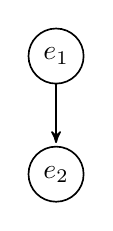
\begin{tikzpicture}[->,>=stealth',shorten >=1pt,auto,node distance=1.5cm,semithick]
            \node[c] (1) [] {$e_1$};
            \node[c] (2) [below of=1] {$e_2$};
            \path[->]
            (1) edge [] node {} (2)
            ;
        \end{tikzpicture}
        }
        \caption{Sequential events (\texttt{seq})}
        \label{encode:cf:seq}
    \end{subfigure}
    ~
    \begin{subfigure}[b]{0.35\textwidth}
        \makebox[\textwidth]{
        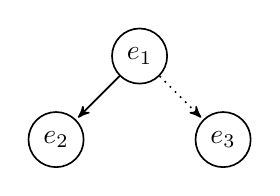
\begin{tikzpicture}[->,>=stealth',shorten >=1pt,auto,node distance=1.5cm,semithick]
            \node[c] (1) [] {$e_1$};
            \node[c] (2) [below left of=1] {$e_2$};
            \node[c] (3) [below right of=1] {$e_3$};
            \path[->]
            (1) edge [] node {} (2)
            (1) edge [dotted] node {} (3)
            ;
        \end{tikzpicture}
        }
        \caption{Conditional branching (\texttt{br})}
        \label{encode:cf:br}
    \end{subfigure}
    ~
    \begin{subfigure}[b]{0.25\textwidth}
        \makebox[\textwidth]{
        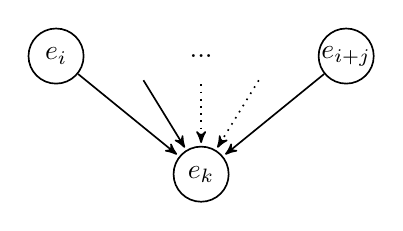
\begin{tikzpicture}[->,>=stealth',shorten >=1pt,auto,node distance=1.5cm,semithick]
            \node[c] (i) [] {$e_i$};
            \node[c,draw=none] (ii) [right=0.2cm of i] {};
            \node[c,draw=none] (iii) [right=0.2cm of ii] {$...$};
            \node[c,draw=none] (iv) [right=0.2cm of iii] {};
            \node[c] (v) [right=0.2cm of iv] {$e_{i+j}$};
            \node[c] (k) [below of=iii] {$e_k$};
            \path[->]
            (i) edge [] node {} (k)
            (ii) edge [] node {} (k)
            (iii) edge [dotted] node {} (k)
            (iv) edge [dotted] node {} (k)
            (v) edge [] node {} (k)
            ;
        \end{tikzpicture}
        }
        \caption{Branch merging (\texttt{mer})}
        \label{encode:cf:merge}
    \end{subfigure}
    %
    \caption{Linear and non-linear cases of control-flow graph}
    \label{encode:cf}
\end{figure}

For listed cases, below we propose the encoding scheme that uniquely encodes each node of graph and allows to encode partially executed program.
Equation~\ref{enc:cf:seq} encodes the sequential control-flow represented in Figure~\ref{encode:cf:seq} and reflects the fact that the event $e_2$ can be executed iff the event $e_1$ has been executed.
Equation~\ref{enc:cf:br} encodes the branching control-flow depicted in Figure~\ref{encode:cf:br} by allowing only following executions: $\{\emptyset, (e_1), (e_1~\rightarrow~e_2), (e_1 ~\rightarrow~e_3)\}$. In encoding~\ref{enc:cf:merge} of the merge-point represented in Figure~\ref{encode:cf:merge}, the event $e_k$ is executed if either of its predecessors was executed, regardless of type of the transition.
%TODO: maybe add the overall formula \phi_{CF} ?

\begin{align}
\phi_{CF_{seq}}   = \ & \fx(e_2) \rightarrow \fx(e_1) \label{enc:cf:seq} \\
\phi_{CF_{br}}    = \ & [\fx(e_2) \rightarrow \fx(e_1)] \land [\fx(e_3) \rightarrow \fx(e_1)] \land \nonumber \\
				  &  [\fx(e_2) \rightarrow \fv(e_1)] \land [\fx(e_3) \rightarrow \lnot\fv(e_1)] \land \nonumber \\
				  & \lnot [\fx(e_2) \land \fx(e_3)]  \label{enc:cf:br} \\
\phi_{CF_{mer}} = \ & \fx(e_k) \rightarrow (\bigvee\limits_{e_p \in \mathtt{pred}(e_k)}^{} \fx(e_p)) \label{enc:cf:merge}
\end{align}


For sake of encoding correctness, we require all branches to have at least one event.
Thus, for branching statements that do not have any events in one of the branches (such a branch represents a conditional jump forward), we add the synthetic \texttt{nop}-event as it is shown in Figure~\ref{encode:branching:nop}:

\begin{figure}[H]
    \centering
    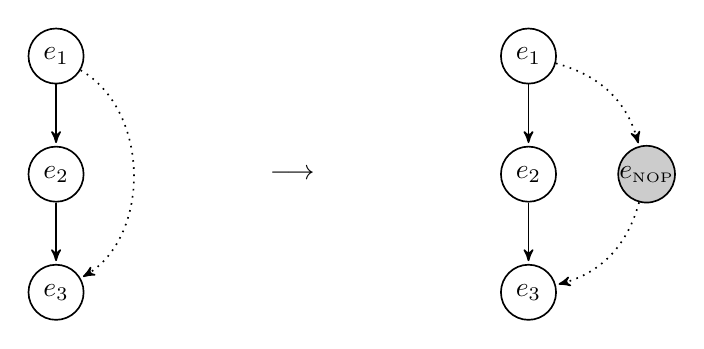
\begin{tikzpicture}[->,>=stealth',shorten >=1pt,auto,node distance=1.5cm,semithick]
        \node[c] at (0,0) (1a) {$e_1$};
        \node[c] at (0,-1.5) (2a) {$e_2$};
        \node[c] at (0,-3) (3a) {$e_3$};
        \node[c,draw=none] at (3,-1.5) (arr) {$\longrightarrow$};
        \node[c] at (6,0) (1b) {$e_1$};
        \node[c] at (6,-1.5) (2b) {$e_2$};
        \node[c,fill=black!20] at (7.5,-1.5) (nop) {$e_{\mbox{\tiny NOP}}$}; %{\tiny{NOP}};
        \node[c] at (6,-3) (3b) {$e_3$};
        \path[->]
        (1a) edge [] node {} (2a)
        (2a) edge [] node {} (3a)
        (1a) edge [dotted,bend left=60] node {} (3a)
        (1b) edge [] node {} (2b)
        (2b) edge [] node {} (3b)
        (1b) edge [dotted,bend left] node {} (nop)
        (nop) edge [dotted,bend left] node {} (3b)
        ;
    \end{tikzpicture}
    \caption{Transformation of the empty-branch nonlinear control-flow}
    \label{encode:branching:nop}
\end{figure}


\subsection{Encoding for the data-flow}
\label{ch:port:enc:df}

To encode the data-flow constraints, we use the \textit{static single-assignment (SSA) form} in order to be able to capture an arbitrary data-flow into a single SMT-formula.
The SSA form requires each variable to be assigned only once within entire program.
In contrast, \porthos used the dynamic single-assignment (DSA) form, that requires indices to be unique within a branch.
Although the number of variable references (each of which is encoded as unique SMT-variable) on average is logarithmically less in case of the DSA form than the SSA form, the result SMT-formula still needs to be complemented by same number of equality assertions when encoding the data-flow in merge points~\cite{Porthos17}.

Following~\cite{Porthos17}, the indexed references of variables are computed in accordance with the following rules:
(1)~any access to a shared variable (both read and write) increments its SSA-index;
(2)~only writes to a local variable increment its SSA-index (reads preserve indices);
(3)~no access to a constant variable or computed (evaluated) expression changes their SSA-index.
These rules determine the following encoding of load, store and computation events within single thread:
%TODO: maybe add the overall formula \phi_{DF} ?
\begin{align}
    \phi_{DF_{e = \mathtt{load}(r \leftarrow l)}} = \ & \fx(e) \rightarrow (r_{i+1} = l_{i+1}) \\
    \phi_{DF_{e = \mathtt{store}(l \leftarrow r)}} = \ & \fx(e) \rightarrow (l_{i+1} = r_i) \\
    \phi_{DF_{e = \mathtt{eval}(...)}} = \ & \fx(e) \rightarrow \fv(e) % \\
\end{align}

To convert the program into SSA form, for each event each variable that is declared so far (either local or shared) is mapped to its indexed reference; this information is stored in the SSA-map "event \textit{to} variable \textit{to} SSA-index". %for each event stores the map that each declared variable maps to its SSA-index
%"$\{$ event : $\{$ variable : index $\}\}$",
%"$\left\{$ event : $\left\{$ variable : index $\right\} \right\}$",
The SSA-map is computed iteratively while traversing the event-flow graph in topological order as it is described in Algorithm~\ref{algorithm:ssa-map}.

\begin{algorithm}
    \caption{Algorithm for computing the SSA-indices}\label{alg:compute-ssa}
    \algorithmicrequire{The event-flow graph $G = \langle N, E \rangle$ where $V$ is the set of nodes (events), $E$ is the set of control-flow transitions, $e_0$ is the entry node}
    \algorithmicensure{The SSA-map of the form "$\{$ event : $\{$ variable : index $\}\}$"}
    \begin{algorithmic}[1]
        \Function{Compute-SSA-map}{G}
            \State {$S \gets$ empty map; $S[e_0] \gets$ empty map}
            \ForAll {event $e_i \in G.N$ in topological order}
                \ForAll {predecessor $e_j \in \mathtt{pred}(e_i)$}
                    \State {$S[e_i] \gets \mathtt{copy}(S[e_j])$}
                    \ForAll {variable $v_k \in$ set of variables accessed by $e_i$ }
                        \State {$S[e_i][v_k] \gets \mathtt{max}(S[e_i][v_k], \ S[e_j][v_k])$}
                        \If {need to update the index of $v_k$} \Comment {cases (1)-(2)}
                            \State {$S[e_i][v_k] \gets S[e_i][v_k] + 1$}
                        \EndIf
                    \EndFor
                \EndFor
            \EndFor
        \EndFunction
    \end{algorithmic}
    \label{algorithm:ssa-map}
\end{algorithm}

The time of described algorithm is linear of the size of event-flow graph since it performs only single traverse of the graph.
%Notwithstanding the overhead of storing (or, equivalently, computing with %TODO: are you sure that 'with'?
%linear time) the predecessors of each node in order to be able to convert the program into an SSA form, the time of such a transformation reduced %TODO: How much ????
%comparing to the algorithm implemented in \porthos, which recomputed SSA-indices recursively for each instruction. %TODO: PROOF OR REMOVE !  Maybe, some words of copying, merging SSA maps ?

As it has been described before, the \rf-relation links data-flow between events %TODO: another word?
of data-flow stored in equivalence assertions over the SSA-variables. 
%The encoding of the \rf-relation, which links the SSA-variables to the original variables, 
The encoding of this linkage left untouched as it is implemented in \porthos: for each pair of events $e_1$ and $e_2$ linked by the \rf-relation, we add the following constraint:

\begin{align}
\phi_{DF_{mem}}(e_1, e_2) = \ & \mathtt{rf}(e_1, e_2) \rightarrow (l_i = l_j) 
\end{align}

where the variable of location $l$ is mapped to the SSA-variable $l_i$ for event $e_1$, and to the SSA-variable $l_j$ for event $e_2$; and the predicate $\mathtt{rf}(e_1, e_2)$ is encoded as a boolean variable, which itself equals $true$ if $e_2$ reads the shared variable that was written in $e_1$.


\subsection{Encoding for the memory model} %Encoding the memory model constraints}
\label{ch:port:enc:wmm}

todo
%Most bounded model-checking problems are solved via computing the fixpoint for the

%The encoding of a weak memory model itself does not depend on the analysing program. The problem here...
%recursive definitions and Kleene iteration

%r 1 ∪r 2 (e 1 , e 2 ) ⇔ r 1 (e 1 , e 2 ) ∨ r 2 (e 1 , e 2 )
%r 1 ∩r 2 (e 1 , e 2 ) ⇔ r 1 (e 1 , e 2 ) ∧ r 2 (e 1 , e 2 )
%r 1 \r 2 (e 1 , e 2 ) ⇔ r W
%r −1 (e 1 , e 2 ) ⇔ r(e 2 , e 1 )
%1 (e 1 , e 2 ) ∧ ¬r 2 (e 1 , e 2 )
%r 1 (e 1 , e 3 ) ∧ r 2 (e 3 , e 2 )
%r ∗ (e 1 , e 2 ) ⇔ r + (e 1 , e 2 ) ∨ (e 1 = e 2 )
%r 1 ;r 2 (e 1 , e 2 ) ⇔
%e 3 ∈E
%r + (e 1 , e 2 ) ⇔ tc ⌈log |E|⌉ (e 1 , e 2 ), where
%tc 0 (e 1 , e 2 ) ⇔ r(e 1 , e 2 ), and
%tc i+1 (e 1 , e 2 ) ⇔ r(e 1 , e 2 ) ∨ (tc i (e 1 , e 2 ); tc i (e 1 , e 2 ))
%
%As it is described in~\cite{Porthos17}, the is based . . .
%~\cite{Porthos17}%, Section "Programs and Memory Models", subsection "Encoding Derived Relations"

\chapter{The~\texttt{porthos2}:~implementation}
\label{ch:impl}

% function invocations/calls: inlining with binding
% contexts: for now, no ctxs
% comparing to cprover (https://www.cprover.org/cbmc/doc/manual.pdf, page 45, absatz about 'goto') where "the loop is unwound a given number of times" , we SHOULD have 2 modes of unrolling: 1) number of times, and 2) number of high-level instructions executed
% TODO(code): (https://www.cprover.org/cbmc/doc/manual.pdf, page 45) "The break and continue statements are replaced by equivalent goto statements as described in the ANSI-C standard."

% TODO: arrays: cprover manual page 48

Current Chapter describes the architecture of the \porthos[2] framework.

The programming language choice for \porthos[2] was made in favour of java in order to be able to reuse some parts of its predecessor \porthos{} written in java.
However this language does not show best results in performance benchmarks (comparing to C++, for example)~\cite{TODO}, the performance cornerstone of \porthos[2] (as well as any other SMT-based code analyser) is the phase of solving the SMT-formula, which is left to the third-party SMT-solver called from \porthos[2] via java API.
However, considering the perspective of using \porthos[2] as a static analyser for real-world programs, the memory optimisation problem must also be taken into account during both encoding and solving stages.



\section{Requirements}
\label{ch:impl:req}

The main reason for starting the work on re-implementing the \porthos{} tool was the need for extension the input language and optimisation of the tool so that it is able to process real C programs in perspective.
In the existing \porthos{} architecture, the high-level recursive instructions (statements of C) are processed together with low-level non-recursive events abstractions (see classes of package `\texttt{dartagnan.program}' of \porthos) as single AST structure.
This AST was implemented as a mutable data structure, which is being modified during the stage of SMT-encoding.
We consider this architecture as hardly manageable (since it is hard to guarantee preserving of the invariants during the program execution) and poorly extensible (since adding support for a new high-level control-flow instruction requires changing multiple components of the program, from parser to encoder).
%Moreover, we encounter serious problems when we need to add support for control-flow jumps (as \texttt{continue}, \texttt{break}, \texttt{goto} in C).

Therefore, while designing the architecture of \porthos[2], we decided to clearly separate the high-level intermediate code representation (implemented as a recursive AST structure) from low-level event-based representation (implemented as an event-flow graph).
Such a modular architecture allows to use multiple input language parsers and convert parsed syntax trees to our AST, thus having support for multiple languages (for instance, the original input language of \porthos{} tool, two variants of syntax of a litmus test used by \tool{herd}, an assembly language for any supported architecture).

The following list enumerates the target \textit{requirements} for the new tool:

\begin{enumerate}[nolistsep]
    \item \textit{stability and transparency}
        \begin{itemize}
            \item following the principles of simplicity and readability;
            \item usage of software design patterns if necessary;
            \item usage of immutable data structures for all data transfer objects~(DTO);
            \item high code coverage by unit and functional tests;
        \end{itemize}
    \item \textit{efficiency}
        \begin{itemize}[leftmargin=1em]
            \item keeping the trade-off between execution time and memory usage;
        \end{itemize}
    \item \textit{extensibility}
        \begin{itemize}[leftmargin=1em]
            \item clear modular architecture
        \end{itemize}
\end{enumerate}



\section{Program Components}
\label{ch:impl:comp}

The general architecture of \porthos[2] is presented in Figure~\ref{fig:program-components}.
The program receives as input the program to be analysed and one (the reachability analysis mode) or two (the portability analysis mode) memory models (see Section~\ref{ch:impl:input-parser}).
Then, the parsed program input (called Y-tree%
\footnote{In order to avoid confusing different internal representations, we prefix the names of elements of each internal representation with a letter. For instance, we picked the letter `Y' to denote the AST code representation as drawing of this letter resembles the tree branching; with letter `X' we prefix elements of the event-flow graph as the events are to be e\textbf{x}ecuted; and with letter `W' we prefix elements of the \textbf{w}eak memory model AST.}%
) is being preprocessed in order to collect information necessary for the compilation (see Section~\ref{ch:impl:y2x:precomp}), and compiled into the X-graph representation (see Section~\ref{ch:impl:y2x:compil}).
If the original program has a loop, the X-graph will have cycles, which need to be unrolled before being encoded into an SMT-formula. The unrolling and some other transformations are made by the X-graph transformer (see Section~\ref{}).

\begin{figure}%[!b]%[H]
  \centering
  \includegraphics[width=\textwidth,height=\textheight,keepaspectratio]{img/my/lucidchart.com/data-flow-vert-300dpi.png}
  \caption{Main components of \porthos[2]}
  \label{fig:program-components}
\end{figure}



%\section{The input language}
%\label{ch:impl:input}
\subsection{Parsing the input}
\label{ch:impl:input-parser}


Both \porthos{} and \porthos[2] \ use the parser generator ANTLR~\cite{parr2013definitive}, a powerful language processing tool.
The full ANTLR grammar of input language used by previous version of \porthos{} is available at Appendix~\ref{apx:in_grammar_pts}.

% TODO: why we've chosen ANTLR (cite Kvanttt); what kind of parser is ANTLR, why it's good for C and not only for C (unified way to define multiple grammars, large collection, ...) + add references

- Figure~\ref{syntax:in_grammar_pts} represents the informal grammar of the input language processed by \porthos[1] ... %todo: cite \cite{Porthos17}.
- short characteristics of the old grammar, enumerate its features (wrt the Figure)

- DRAWBACKS: %what parts need to be improved:

    -- the semantics of memory operations and method invocations is encoded directly into the grammar.
    Taking into account the complexity of developing the accurate grammar for a Turing-complete language,

    -- in old implementation, the logics of parser was written directly in the grammar.
    Although being fast-to-impelement (1 internal representation less), this is approach has numerous drawbacks s.a.:
    * hard to read grammar (mixing 2 languages in a single file)
    * hard to maintain grammar (no debugging with standard utils, no code analysis in the grammar file)
    * non-extensible (there is no option to just plug-in existing grammar for any language and write a converter from this language's syntax tree to our AST)

    - syntactically only the integers were supported. we:arrays???pointers??enums?structs?

    - no declarations (all shared variables are declared in the init section, local variables are not decalred ever)

    - no arbitrary function calls (need support for the knowledge base after implementing the typisation. cannot be supproted only syntactically)


- Minor drawbacks:

    - restricted sytnax for expressions:

    -- no operator associativity allowed (`1 + 2 * 3` was invalid syntax)

    -- no unary increment/decrement (technically it's hard to implement post-incerment/decrement without interpretation: we don't know when does this expression ends.)
    Example:
    `int* x;
    if (x++ > 0 ) { }`
    % todo: test pre-/post-fix operations //+think how current tool will behave if there's more than one post-operation //and pre-operation

    -- incorrectly implemented statement in old code: sequence of stmts is separated by ';', but the syntax of C requires ';' as the operator that ends each operation (how to say this? see C standard)

    -- litmus-initialisation  stmt did not allow the non-default values. The new syntax allow any type of declaration statement with initialisation

- this means the full compiler engine that resolves the semantics

%The grammar supported by \porthos[2] was extended in order to support expressions valid in C. %TODO: examples, how imenno extended
%Also, the input language of the first version of \porthos{} syntactically distinguished the type of a memory instruction (shared variable assignments were defined with symbol~`\texttt{:=}', and local variable assignments --- with symbol~`$\mathtt{\leftarrow}$'), whereas \porthos[2] determines the semantics of a function invocation during the preprocessing stage of compilation~(see Chapter~\ref{TODO!!!}).

% todo: this is the simplified grammar

%TODO: although the grammar is context-free and fail whith <angle brackets>.... it still works fine. Even gcc uses CF grammar? reference to INRIA's parser and paper on discussing grammars for C

%TODO: say sth about 100500 litmus-tests for kernel

\begin{figure}%[H]
%\begin{multicols}{2}
\begin{lstlisting}[mathescape=true,%
                  caption={Syntax of an input language of \porthos{} version 1},%
                  label={syntax:in_grammar_pts},%
                  %literate={<--}{{$\leftarrow$}}1,%
                  morekeywords={if,then,else,return,while,program,thread}%
                  breaklines=true,%
                  basicstyle=\ttfamily\scriptsize]
<prog> : <init> <thrd>* <assert>
       ;
<thrd> : thread <tid> <inst>
       ;
<inst> : <atom>
       | <inst> ; <inst>
       | while <pred> <inst>
       | if <pred> { <inst> } <inst>
       ;
<atom> : <reg> <-- <expr>
       | <reg> <-- <loc>
       | <loc> := <reg>
       | 'mfence'
       | 'sync'
       | 'lwsync'
       | 'isync'
       ;
<pred> :
       | true
       | false
       | <expr> (and | or) <expr>
       | <expr> ('==' | '!=' | '>' | '>=' | '<' | '>=') <expr>
       ;
<expr> : [0-9]
       | <reg>
       | <expr> ('*' | '+' | '-' | '/' | '%') <expr>
       ;
\end{lstlisting}
%\end{multicols}
\end{figure}


- NOW: we're using the C grammar from the standard

- for now, we just ignore C macro directives, in future it's planned to support partially the preprocessing before parsing

The \porthos[2] uses the C language grammar of proposed in the C11 standard~\cite{jtc2011sc22}, that was extended by litmus test-specific syntax such as initialisation and final-state assertion statements (the original ANTLR grammar can be found in the official ANTLR repository on GitHub~\footnote{The repository containing the collection of ANTLR v4 grammars:\\ \url{https://github.com/antlr/grammars-v4}}).
Current version of \porthos[2] can operate only in the inter-procedural mode, assuming that each function defined in the input file is being executed in a separate thread.
However, the redesigned architecture of \porthos[2] allow to easily support intra-procedural analysis by inlining function calls.

%TODO: say sth about syntax errors handling: still now, what if parser does not accept syntax?

- if we don't support , our parser still parses it, and the error is thrown at the moment of converting syntax tree to the AST (Y-tree).

- So, The language-dependent syntax tree is converted to the AST by the stateless Visitor (e.g., for C11->Ytree conversion is made by 'C2YtreeConverterVisitor') + short structure of this visitor (how?.. need ly?)


\section{The Y-tree: an AST}
\label{ch:impl:ytree}

- picture of the Y-hierarchy. everything inherits interface YEntity

- immutable

- AST is untyped (YVariableRef).

- short characteristics with citations from the code (this AST contains very basic language elements according to the C execution model (statements and expressions) )

- minor changes are performed by converting to ytree representation: desugaring the target code, etc. (what else?)


\section{Model parser}
\label{ch:impl:model}

TODO


\section{Compiling the Y-tree to the X-graph}
\label{ch:impl:y2x}

%todo: some words on necessity of contexts and lack of them. How would we implement them

%todo: rename Interpreter -> Compiler.

%note https://en.wikipedia.org/wiki/Semantics_(computer_science)
%Operational semantics loosely corresponds to interpretation,

- hierarchy of Compilers (XCompiler is an stateful abstract machine)

- interface that it provides

- dependencies on other modules (memory-manager, etc.)


\subsection{Pre-compilation}
\label{ch:impl:y2x:precomp}

- collect goto labels (not done yet.)

- determine kind of variables (cannot be done during parsing? don't say this)

- basic typisation

%todo: after all, list which modules (classes, managers) are being initialised during the pre-compilation. I'ts good to have the dependencies graph on moduls (operational semantics:) )

\subsection{Compilation}
\label{ch:impl:y2x:compil}

- more low-level code representation (or high-level assembly); abstract assembly language. refer to the %2_wmm.tex

- X-hierarchie


\subsection{Post-compilation transformations}
\label{ch:impl:x2y:postcomp}

- After we acquired the event-based representation, we can perform some modifications/simplifications/optimisations on it (separately, allowing user to manage them)

- converting to SSA form (now: during the encoding. should be: during the post-compilation) (as one of necessary steps before encoding)

- setting up backward edges

- more?

- unrolling: why we cannot encode cyclic structures. reference to the paper (see arXiv version)
% If the analysing program contains a loop, then its control-flow graph represents the cyclic directed graph. Although, in order to be able to encode such a cyclic structure as a boolean formula, this graph needs to be

The original program encoded into the \texttt{XGraph} represents a \textit{flow graph}, a connected cyclic directed graph with single source node \texttt{(ENTRY)} (usually for convenience all leaves are connected to the sink node \texttt{(EXIT)}). The cycles are caused by low-level jump instructions, obtained from non-linear high-level control-flow statements (such as \texttt{while}, \texttt{do-while}, \texttt{for}, etc.). However, the cyclic flow graph cannot be encoded into SMT formula since ...
//TODO:REFERENCE.%TODO



\begin{figure}
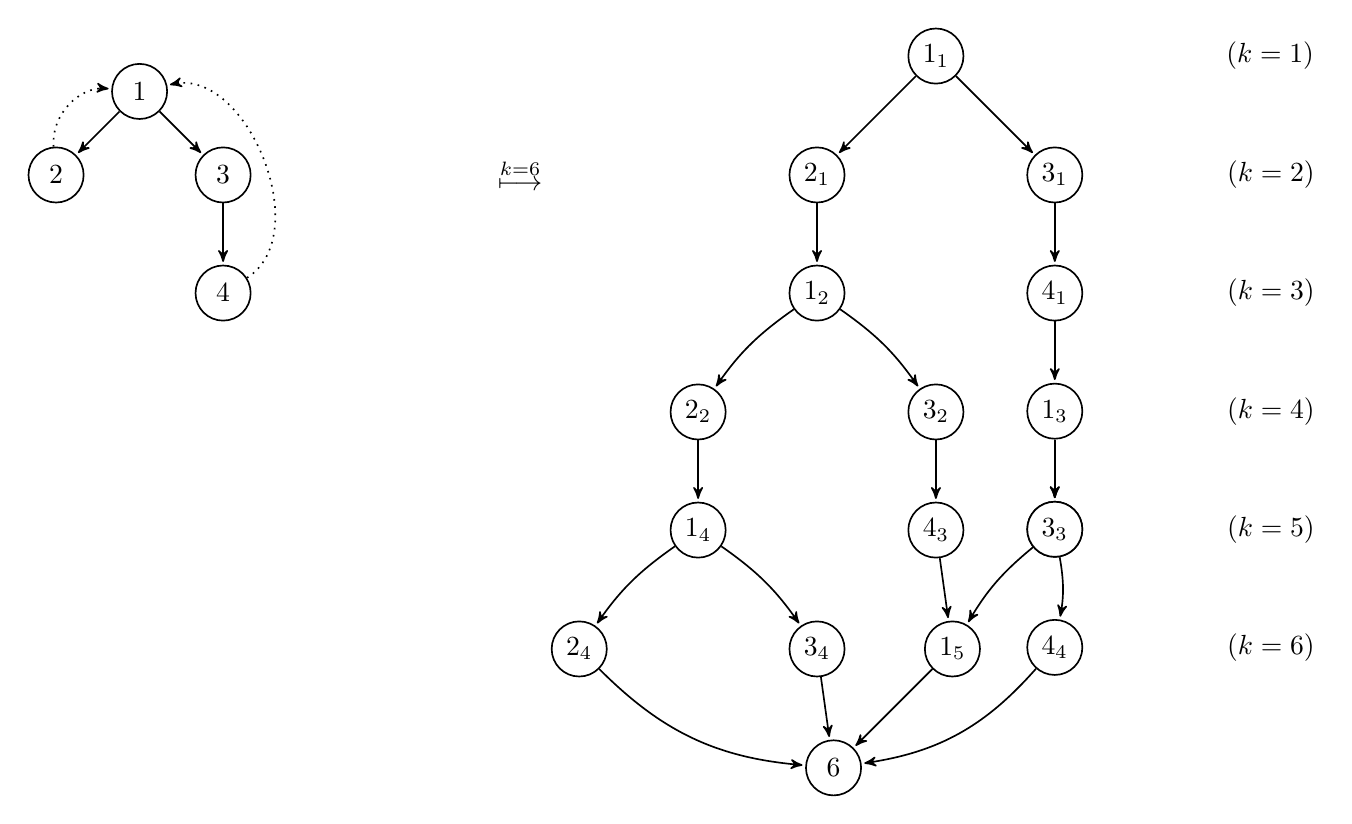
\begin{tikzpicture}[->,>=stealth',shorten >=1pt,auto,node distance=1.5cm,semithick]
\node[c] (1) [] {$1$};
\node[c] (2) [below left of=1] {$2$};
\node[c] (3) [below right of=1] {$3$};
\node[c] (4) [below of=3] {$4$};
\path[->]
(1) edge [] node {} (2)
(2) edge [bend left=50,dotted] node {} (1)
(1) edge [] node {} (3)
(3) edge [] node {} (4)
(4) edge [bend right=80,dotted] node {} (1)
;
\node[draw=none] (impl) [right=3cm of 3] {$\overset{k = 6}{\longmapsto}$};
;
\node[c] (21) [right=3cm of impl] {$2_1$};
\node[c] (11) [above right=1cm and 1cm of 21]{$1_1$};
\node[c] (31) [below right=1cm and 1cm of 11] {$3_1$};
\node[c] (41) [below of=31] {$4_1$};
\node[c] (12) [below of=21] {$1_2$};
\node[c] (22) [below left=1cm and 1cm of 12] {$2_2$};
\node[c] (32) [below right=1cm and 1cm of 12] {$3_2$};
\node[c] (13) [below of=41] {$1_3$};
\node[c] (14) [below of=22] {$1_4$};
\node[c] (43) [below of=32] {$4_3$};
\node[c] (23) [below of=13] {$2_3$};
\node[c] (33) [below of=13] {$3_3$};
\node[c] (24) [below left=1cm and 1cm of 14] {$2_4$};
\node[c] (34) [below right=1cm and 1cm of 14] {$3_4$};
\node[c] (15) [below right=1cm and -0.3cm of 43] {$1_5$};
\node[c] (44) [below of=33] {$4_4$};
\node[c] (6) [below left=1cm and 1cm of 15] {$6$};
\node[] (11k) [right=3.2cm of 11] {$(k = 1)$};
\node[] (31k) [right=1.7cm of 31] {$(k = 2)$};
\node[] (41k) [right=1.7cm of 41] {$(k = 3)$};
\node[] (13k) [right=1.7cm of 13] {$(k = 4)$};
\node[] (33k) [right=1.7cm of 33] {$(k = 5)$};
\node[] (44k) [right=1.7cm of 44] {$(k = 6)$};
\path[->]
(11) edge [] node {} (21)
(11) edge [] node {} (31)
(31) edge [] node {} (41)
(21) edge [] node {} (12)
(12) edge [bend right=10] node {} (22)
(12) edge [bend left=10] node {} (32)
(41) edge [] node {} (13)
(22) edge [] node {} (14)
(32) edge [] node {} (43)
(13) edge [] node {} (23)
(13) edge [] node {} (33)
(14) edge [bend right=10] node {} (24)
(14) edge [bend left=10] node {} (34)
(43) edge [] node {} (15)
(33) edge [bend right=10] node {} (15)
(33) edge [bend left=10] node {} (44)
(24) edge [bend right=20] node {} (6)
(34) edge [] node {} (6)
(15) edge [] node {} (6)
(44) edge [bend left=20] node {} (6)
;
\end{tikzpicture}
\label{fig:loop-unwind}
\caption{Example of the flow graph from Figure~\ref{fig:merged-loop.....}, unwinded up to the bound $k = 6$}
\end{figure}




\section{XGraph to ZFormula (SMT) encoder}
\label{ch:impl:comp:zformula}

- Then, this modified event-representation is being encoded to SMT formula and sent to the solver.



% say something about equals() and hashCode()



\section{Optimisations}

... performed on each stage
\chapter{Evaluation}
\label{ch:eval}

tests


\section{Comparison with \porthos{}}

\subsection{Performance}

- enc-time absolute values
- rate enc-time/solve-time



\section{Comparison with HERD}

\subsection{Unique Features}

\subsection{Performance}


\chapter{Conclusion}
\label{ch:summary}


\section{Solved tasks and contributions}

During the work on this thesis, we solved the following engineering and scientific tasks:

\begin{enumerate}[label=\Roman*.]
\item
Firstly, we studied existing weak memory model-aware analysis frameworks and tools to gather deep understanding of the problem (Sections~\ref{ch:intro:related} and~\ref{ch:enc:mc} and Chapter~\ref{ch:wmm}).

\item
Then, we explored the existing implementation of the proof-of-concept tool \porthos[1] in order to understand components that need to be redesigned in order to facilitate the extension of the input language.

  \begin{enumerate}[label=\roman*.,leftmargin=\parindent]
  \item The first stumbling block in the input language extension was the \porthos[1] input language parser, which performs the full semantic analysis of the program.
  Although this works for a small toy language, the rich and expressive language such as C requires several stages of analysis before the compilation stage.
  For handling that, we implemented the processing units that operate on the \textit{pre-compilation} stage discussed in Section~\ref{ch:impl:proc:x-pre-compiler}.
  
  \item Secondly, as \porthos[2] determines the \textit{kind (shared or local) of each variable} on the pre-compilation phase, the shared variables can be accessed in arbitrary code location (comparing to \porthos[1] which determines the type of a variable syntactically, depending on the operator of function that uses the variable).
  
  \item In addition, \porthos[2] supports some \textit{new syntactic constructions} of the C language: \texttt{break} and \texttt{continue} jumps, function invocations, multiple-variable declarations (as `\texttt{int a, b=2, z;}'), arbitrary expressions (corresponding to the C standard), and others (see Section~\ref{ch:impl:input}).

  \item As the C language supports unconditional \texttt{goto}-jumps that can produce an arbitrary control-flow graph, which cannot be supported solely with the program AST, therefore we needed to compile the AST to the low-level hardware-agnostic program representation \xgraph{}.
  For that, we implemented the \textit{full C interpreter} discussed in Section~\ref{ch:impl:proc:x-compiler}.
  
  \item Originally, the control-flow instructions were encoded directly into the SMT-formula~\cite{Porthos17a}.
  In contrast, \porthos[2] encodes the low-level \xgraph{} representation, which can have arbitrary graph structure.
  For encoding the \xgraph{} into the SMT-formula, we apply the \textit{new control-flow encoding scheme} that in general follows the one proposed in~\cite[Chapter 5.1.2]{heljanko2008unfoldings} (see Section~\ref{ch:enc:bmc:cf}).
  As the new encoding scheme does not add new variables to every control-flow instruction, the number of variables in the result SMT-formula is expected to be smaller.
  
  \item For ease the process of adding support for new domain-specific functions (for example, the Kernel-specific atomic write function \texttt{atomic\_store}), we implemented the \textit{invocation hooking}, a flexible mechanism for intercepting the compilation process without changing the interpreter.
  The invocation hooking mechanism serves as a knowledge base for the program domain, that is to be filled and extended in future.
  Invocation hooks are defined in Java and thus are flexible, though their extension and modification requires some knowledge of the internals of the tool.
  We illustrate this mechanism with the basic support for Linux kernel litmus tests.
  
  \item Since the new tool compiles the program AST to the \xgraph{} before encoding it into the SMT-formula, we decided to change the \textit{unrolling algorithm} from the simple unrolling all loops $k$ times (where $k$ is the user-specified unrolling bound) to the DFS-based algorithm that explores all possible states that the program can reach within $k$ steps (see discussion on the unrolling in Sections~\ref{ch:impl:proc:x-unroll} and~\ref{ch:eval:show:compil}).
  Although the new algorithm produces considerably more events than the old algorithm and thus the requires more time for the program domain encoding, we claim it to be complete.
  
  \end{enumerate}
  
\item 
As the tests show, the overhead of the new architecture is negligible, therefore we consider the applied architectural changes as acceptable.

\end{enumerate}

Thus, the new tool \porthos[2] with easily extensible knowledge base that allow to support new domain-specific functions can be considered as a generalised framework for SMT-based memory model-aware analysis.

%enumerate goals (from Task specification) in past tense + justification


\section{Limitations and future work}

Current implementation of \porthos[2] has the following limitations, that might define the direction of the future work.

\begin{itemize}
\item The major flaw of \porthos[2] as a tool that performs the complete software analysis is the its sensitivity to the combinatorial explosion.
%TODO: show it in table , reference here the table
As it was shown in Section~\ref{ch:eval:perf}, the number of events generated by the program grow rapidly as the user increases the unrolling bound.
One possible way to reduce the number of states of the program might be applying some traditional techniques for fighting the state explosion problem (such as concrete execution as a part of concolic execution~\cite{majumdar2007hybrid}), however this must be done \textit{with considering the weak memory model}, because otherwise it could possibly lead to the loss of states.
% cannot be applied to our problem \textit{before} the weak memory model is considered, 
%One possible enhancement, that could treat but not cure this flaw, could be an extra analysis stage carried before the unrolling, that analyses 

%\item As its predecessor, \porthos[2] does not propose any heuristic for finding the optimal unrolling bound.

\item As its predecessor, \porthos[2] 

\end{itemize}

%- improve the encoding: an abstraction over Z
- testing with new solvers

- typing: const-size arrays + structures and so on
  -only basic datatypes

%- hooks : flexible. but still in Java, not as separate module (as it requires turing-complete language to be expressive enough) => extension of the knowledge base for supporting new platforms / languages

- new modes: as it was discussed <before>, works only in the litmus test-mode. May work with complete projects. But here: 
  - memory issues (we store same graph + back edges + memoised queries ==> multiple instances.);
    - + will need the memory-guarding module
  - ability to encode partially (once the 

-only one mode litmus-test intra proc



% Fix numbering of bibliography section
\cleardoublepage
\phantomsection

\addcontentsline{toc}{chapter}{\bibname}

\printbibliography
%% And now the sub-bibliographies: we use three of them (based on the entry type). Each sub-bibliography assigns a different prefix. The option is called 'prefixnumbers' because it was originally intended for numeric citations only. It also works with alphabetic labels:
%\printbibliography[heading=subbibliography,title={Articles},type=article]%,prefixnumbers={A-}]
%\printbibliography[heading=subbibliography,title={Books},type=book]%,prefixnumbers={B-}]
%\printbibliography[heading=subbibliography,title={Collections},type=collection]%,prefixnumbers={C-}]

% Appendices go here
% ------------------------------------------------------------------
% Fix numbering of bibliography section
%\cleardoublepage

\renewcommand{\thesection}{A.\arabic{section}}
%\titlespacing*{\section}{0pt}{-40pt}{20pt}
\titlespacing*{\section}{0pt}{0pt}{0pt}
\titleformat{\section}[display]
  {\normalfont\large\bfseries}% <- font for label "A.1", default \huge
  {}
  {0ex}
  {\thesection\quad\large}
\newcommand{\sectionbreak}{\clearpage}

\cleardoublepage\makeatletter\@openrightfalse\makeatother
\phantomsection
\appendix
\addcontentsline{toc}{chapter}{Appendices}
\fancyhead[R]{\footnotesize\itshape{APPENDICES}}
\appendixpage

%\vspace{-3em}
%TODO: grammar highlight with bold font!
%\begin{figure}[h!]%[H]
\begin{multicols*}{2}
[
\section{The ANTLR grammar for the \texttt{porthos\,v1} input language}
\label{apx:grammar}
]
\begin{lstlisting}[language=antlr,
        basicstyle=\tiny,
        linewidth=.56\textwidth]
grammar Porthos;

main
  :   program
  ;

bool_expression
  :   bool_atom
  |   bool_atom BOOL_OP bool_atom
  ;

bool_atom
  :   TRUE
  |   FALSE
  |   '(' arith_expr COMP_OP arith_expr ')'
  |   '(' bool_expression ')'
  ;

arith_expr
  :   arith_atom ARITH_OP arith_atom
  |   arith_atom
  ;

arith_atom
  :   DIGIT
  |   register
  |   '(' arith_expr ')'
  ;

register
  :   WORD
  ;

location
  :   WORD
  ;

local
  :   register '<-' arith_expr
  ;

load
  :   register '<:-' location
  ;

store
  :   location ':=' register
  ;

read
  :   register '=' location '.' 'load' '(' 
     ATOMIC ')'
  ;

write
  :   location '.' 'store' '(' ATOMIC ',' 
     register ')'
  ;

instruction
  :   atom
  |   sequence
  |   while_
  |   if
  ;

atom
  :   local
  |   load
  |   store
  |   FENCE
  |   read
  |   write
  ;

sequence
  :   atom    ';' instruction
  |   while_  ';' instruction
  |   if      ';' instruction
  ;

if
  :   'if' bool_expression 'then' '{' instruction '}' 
     ('else' '{' instruction '}')?
  ;

while_
  :   'while' bool_expression '{' instruction '}'
  ;

program
  :   '{' location (',' location)* '}'
       ('thread t' DIGIT '{' instruction '}'
         ('exists' (location '=' DIGIT ','
         | DIGIT ':' register '=' DIGIT ',')   
         )*
       )*
  ;

// Lexer rules:

ATOMIC
  :   '_na' | '_sc' | '_rx' | '_acq' | '_rel' | '_con'
  ;

FENCE
  :   'mfence' | 'sync' | 'lwsync' | 'isync'
  ;
    
COMP_OP  : '=='  | '!='  | '<=' | '<' | '>=' | '>';
ARITH_OP : '+'   | '-'   | '*'  | '/' | '%';
BOOL_OP  : 'and' | 'or';

DIGIT  : [0-9];
LETTER : 'a'..'z' | 'A'..'Z';
TRUE   : 'true'   | 'True';
FALSE  : 'false'  | 'False';
WORD   : (LETTER | DIGIT)+;
\end{lstlisting}
\end{multicols*}
%\end{figure}


%\begin{multicols*}{2}
%[
%\section{The ANTLR grammar for the \texttt{cat} language}
%\label{apx:catgrammar}
%]
%\lstinputlisting{inc/lst/grammars/Cat.g4}
%\end{multicols*}
\section{File trees of \texttt{Y-tree} and \texttt{X-graph} representations}
\label{apx:trees}

\hspace*{\fill}%
\begin{minipage}[t]{0.55\textwidth}
  \VerbatimInput{inc/lst/Ytree-tree.out}
  %\includegraphics[width=\textwidth]{1.png}
  %\caption{Picture 1}
  %\label{fig:1}
\end{minipage}
\hfill%
\begin{minipage}[t]{0.35\textwidth}
  %\begin{flushright}
  \VerbatimInput{inc/lst/Xgraph-tree.out}
  %\end{flushright}
  %\caption{Picture 2}
  %\label{fig:2}
\end{minipage}
\hspace*{\fill}%
\section{The simplified x86-TSO memory model defined in the \cat{} language~\cite{herd10tutorial}}
\label{apx:x86cat}

\begin{figure}[h]
\begin{lstlisting}
"X86 TSO"
include "x86fences.cat"
include "filters.cat"
include "cos.cat"

(* Uniproc check *)
let com = rf | fr | co
acyclic po-loc | com

(* Atomic *)
empty rmw & (fre;coe)

(* Global happens-before *)
#ppo
let po_ghb = WW(po) | RM(po)

#mfence
include "x86fences.cat"

#implied barriers
let poWR = WR(po)
let i1 = MA(poWR)
let i2 = AM(poWR)
let implied = i1 | i2

let com = rfe | fr | co
let ghb = mfence | implied | po_ghb | com
show implied
acyclic ghb as tso
\end{lstlisting}
%\caption{\protect\footnotemark}
%\label{example:x86-cat}
\end{figure}
\section{Public interface methods of the X-interpreter}
\label{apx:xinterpreter}

%\begin{figure}[h]
\lstinputlisting[language=Java,linewidth=1.1\textwidth]{inc/lst/XInterpreter.java}
%\end{figure}


% End of document!
% ------------------------------------------------------------------
% The LastPage package automatically places a label on the last page.
% That works better than placing a label here manually, because the
% label might not go to the actual last page, if LaTeX needs to place
% floats (that is, figures, tables, and such) to the end of the
% document.
\end{document}

